\documentclass[14pt, a4paper]{article}
\usepackage[russian]{babel}
\usepackage{graphicx}
\usepackage{layout}
\usepackage[14pt]{extsizes}

\setcounter{tocdepth}{4}
\setcounter{secnumdepth}{4}

\usepackage{xcolor}
\usepackage{hyperref}

 % Цвета для гиперссылок
\definecolor{linkcolor}{HTML}{000000} % цвет ссылок
\definecolor{urlcolor}{HTML}{000000} %цвет гиперссылок

\hypersetup{pdfstartview=FitH,  linkcolor=linkcolor,urlcolor=urlcolor, colorlinks=true}
\definecolor{backcolour}{rgb}{0.97,0.97,0.97}
% \renewcommand{\section}{Глава}
% \usepackage{emoji}
% \setemojifont{Apple Color Emoji}



\oddsidemargin = 0pt
\marginparwidth = 45pt %57
\textwidth = 467pt
\textheight = 716pt
\topmargin = 0pt %17
\footskip = 30pt %30
\headheight = 0pt %12
\headsep = 0pt %25

% \setcounter{tocdepth}{1}

\begin{document}
\begin{titlepage}
    \topmargin=216pt
    \newpage
    \hangindent=0.7cm
    \huge ИУ-10\\
    Системное\\
    Программное\\
    Обеспечение\\
    Системы виртуализации\\
    \textbf{Гипервизоры второго типа\\
    (интегрированные с \\хост-системой)}

    \vspace{10cm}

    \begin{center}
        \small\textit{Москва, 2022}
    \end{center}
\end{titlepage}

\section*{На этом уроке}
\begin{enumerate}
    \item Изучим общие особенности гипервизоров второго типа.
    \item Рассмотрим примеры их реализации: VMware Workstation, VMware Fusion, Oracle VirtualBox.
\end{enumerate}

\tableofcontents
\vspace{1cm}

Гипервизоры, интегрированные с хост-системой, первыми получили широкое распространение. По
сути, гипервизор — обыкновенное приложение, запущенное поверх основной операционной системы.
Данный подход менее эффективен по сравнению с запуском гипервизора непосредственно на
аппаратуре, однако он всё ещё широко используется благодаря простоте установки и
администрирования, а также своим привлекательным особенностям:

\begin{itemize}
    \item простому взаимодействию с основной ОС (разделяемые папки и буфер обмена);
    \item возможности проброса некоторых устройств, таких как GPU и USB, в виртуальную машину.
\end{itemize}

Может показаться несколько странным, что рассмотрение реальных гипервизоров мы начинаем с
гипервизоров второго типа, а вовсе не первого — их мы рассмотрим на следующем занятии. Из
экскурса в историю развития систем виртуализации вы помните, что в 60–70-е годы прошлого
столетия инженеры компании IBM придумали и реализовали концепцию виртуализации mainframe.
Успех их разработки во многом основывался на том, что IBM имела контроль и над программным
обеспечением, и над аппаратурой, для которой это ПО создавалось. Гипервизор, впервые созданный
в IBM, работал непосредственно на процессоре без дополнительных прослоек ПО. Это и называется
гипервизором первого типа.\\

Такой подход долгое время был невозможен в мире x86. Компании-разработчики процессоров (в
основном Intel и AMD) были в большей мере озабочены разработкой, производством и продажей
процессоров, нежели разработкой ПО для них. ПО для компьютеров с архитектурой x86
разрабатывали сторонние компании, которым приходилось мириться с недостатками аппаратуры.\\

Более того, независимые разработчики ПО не имели возможности или желания разрабатывать
полный спектр ПО, предпочитая сконцентрировать усилия в какой-то одной области. Так, например,
компания Microsoft занималась разработкой операционных систем и офисных приложений. А группа
молодых инженеров из Стэнфорда решила сконцентрироваться на развитии своего научного проекта
Disco, создав компанию VMware. И первый коммерческий продукт VMware был реализацией
гипервизора второго типа, работающего поверх имеющейся операционной системы.\\

Ниже приведена блок-схема гипервизора второго типа, наглядно демонстрирующая полную
вычислительную систему с запущенным гипервизором второго типа.

\begin{figure}[h]
    \centering
    \scalebox{0.9}{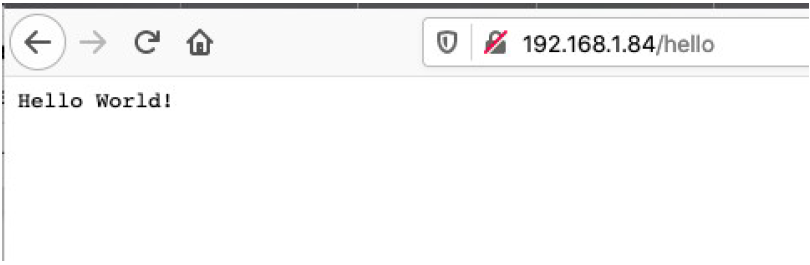
\includegraphics[width=1\textwidth]{2.png}}\\
    \label{framework} 
\end{figure}

Из этой блок-схемы видно, что гипервизор мало чем отличается от любых других приложений,
запущенных хозяйской операционной системой, например, текстового редактора. В частности, как и
другие приложения, гипервизор использует сервисы, предоставляемые ОС: виртуальную память,
доступ к хранилищам данных, сетям обмена данными и т. д. То есть соответствующую
функциональность не нужно реализовывать как часть гипервизора, что неизбежно в случае
гипервизора первого типа. Это позволяет сконцентрироваться на разработке основной
функциональности виртуальной машины — создании и поддержании виртуализированного окружения.\\

Ещё одно важное преимущество такого подхода — высокая переносимость гипервизора между
разными компьютерами. Поскольку средствами имеющейся ОС происходит абстрагирование от
реальной аппаратуры конкретного компьютера, достаточным условием для успешного запуска
гипервизора в самом простом случае оказывается наличие определённой ОС.\\

Это условие остаётся достаточным до тех пор, пока гипервизор осуществляет полную бинарную
трансляцию или эмуляцию всех команд гостевого ПО. Если же хоть какая-то часть ПО гостевой
системы выполняется непосредственно на реальном процессоре в системе, дополнительным
условием становится совпадение наборов команд (ISA — Instruction Set Architecture) хозяйской и
гостевых систем.
\newpage


\section*{Общие особенности}
\addcontentsline{toc}{section}{Общие особенности}

\subsection*{Установка}
\addcontentsline{toc}{subsection}{Установка}

Многим продвинутым пользователям персонального компьютера знакомо такое упражнение:
установить на домашний или даже рабочий компьютер одну из двух доступных бесплатно
виртуальных машин и в виртуальной машине установить какой-то популярный Linux-дистрибутив.
Обычно речь идёт об Ubuntu, но вполне могут быть и альтернативные варианты.\\

Причин проделать это упражнение может быть несколько. Например, необходимость запуска
недоступной для Windows программы или пакета программ, взять хотя бы LAMP-стек. LAMP —
сокращение от Linux, Apache, MariaDB/MySQL, PHP. Ещё одна возможная причина — желание
познакомиться с незнакомой ОС ввиду её всё большей популярности. А может быть, хочется
поэкспериментировать с установкой и настройкой ОС перед опытами над реальным бабушкиным
компьютером в безопасном окружении, песочнице.\\

Любой описанный выше сценарий легко осуществим при помощи Oracle Virtualbox или VMware Player,
поскольку для пользователя установка и настройка обоих инструментов мало чем отличается от
установки и запуска любой другой программы. Установщик можно без каких-либо сложностей
загрузить с веб-сайта производителя, а после загрузки достаточно запустить его на выполнение. Не
забудьте внимательно прочитать лицензионное соглашение перед нажатием кнопки «Согласен».
Через пару окошек и несколько минут всё готово для работы с виртуальной машиной.
\newpage

\subsection*{Настройка}
\addcontentsline{toc}{subsection}{Настройка}

\begin{figure}[h]
    \centering
    \scalebox{1}{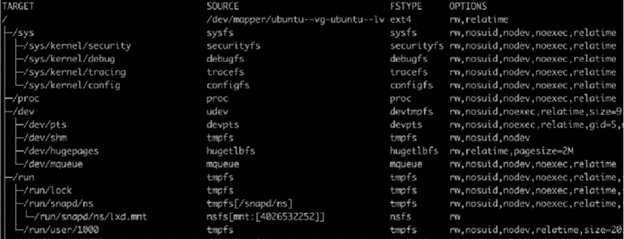
\includegraphics[width=1\textwidth]{3.png}}\\
    \label{framework} 
\end{figure}

Немного более сложной может показаться настройка виртуальной машины. Но и тут, если
использовать предложенные по умолчанию значения, процесс может выглядеть как последовательное
нажатие кнопки «Далее». Теперь нажимаем «Запуск», и виртуальная машина начала работу.\\

Для обывателя всё выглядит невероятно просто и удобно. Для системных администраторов, которые
занимаются поддержкой такого рода виртуальных машин, доступны средства управления из
командной строки. Это значит, что возможно удалённое управление парком виртуальных машин, а
также скриптование и автоматизация некоторых задач: запуска и остановки, создания снимков
состояния ВМ.\\

И всё-таки разберёмся, что нужно настраивать и зачем. По определению виртуальная машина —
модель некой реальной аппаратуры, которая обладает определёнными свойствами, зависящими от
составляющих её компонентов. Например, от типа и количества центральных процессоров, объёма
оперативной памяти, типа и объёма постоянного накопителя данных (дисковый или твердотельный),
типа и количества дополнительных периферийных устройств, таких как сетевые контроллеры, USB и
т. д.\\

Современные системы виртуализации позволяют пользователю достаточно гибко выбирать
конфигурацию ВМ. Может возникнуть вопрос: а зачем вообще заниматься настройкой, почему бы не
использовать универсальную конфигурацию? Во-первых, может стоять задача максимально точной
эмуляции какой-то конкретной системы. А во-вторых, у пользователя есть возможность гибко и
осмысленно распорядиться ресурсами своей системы: выделить виртуальной машине достаточно ресурсов для выполнения предполагаемых задач, оставив хозяйской системе достаточно ресурсов
для продолжения комфортной работы. Если это имеет значение! Вполне возможно, что нам бы
хотелось передать ВМ если не все ресурсы хозяйской системы, то их максимальное количество,
чтобы максимально быстро выполнить какую-то работу.\\

Как правило, есть возможность указать следующие параметры:
\begin{enumerate}
    \item \textbf{Количество процессорных ядер хозяйской системы, доступное гостевой системе.} Этот
    параметр имеет значение для систем с многоядерными процессорами или же с несколькими
    процессорами. Выделяя заданное количество ядер, можно гибко делить общую
    вычислительную мощность хозяйской системы между задачами в хозяйской системе и
    гостевыми окружениями. Например, при наличии процессора с четырьмя ядрами можно
    запустить две виртуальные машины, выделив первой одно ядро, второй — два ядра, и одно
    оставив в пользовании хозяйской системы.
\end{enumerate}

\noindent Как правило, такую конфигурацию имеют высокопроизводительные серверы. В персональных
компьютерах, если только это не высокопроизводительная рабочая станция, в настоящее время
используются процессоры с одним, двумя или четырьмя вычислительными ядрами. Стоит отметить,
что процессоры, реализующие аппаратную многопоточность, интерпретируются современными
операционными системами как многоядерные системы с большим количеством ядер. В терминологии
Intel это Hyperthreading, на языке AMD — Simultaneous MultiThreading, SMT.\\

Сегодня в широко распространённых процессорах реализуют два аппаратных потока выполнения, то
есть ОС может отображать количество доступных для аллокации процессорных ядер от одного до
восьми (четыре ядра, по два потока на каждом).\\

Не стоит, однако, думать, что выделенные гостевым системам ядра реального процессора
оказываются как-то по-особенному привязаны к гостевой системе и уж тем более становятся
полностью недоступны для обслуживания хозяйской ОС и процессов, запущенных в ней. Количество
«выделенных» ядер лишь информирует гипервизор о том, что можно использовать N потоков
выполнения. Но только хозяйская ОС занимается реальной диспетчеризацией задач, в том числе и
потоков выполнения гипервизора, на реальные вычислительные ядра.
\begin{enumerate}

\item[2.] \textbf{Максимальный объём оперативной памяти, который гостевая система может
использовать.} В чём-то этот параметр похож на предыдущий: он информирует гипервизор о
том, какой объём памяти можно запросить у хозяйской системы. И так же, как и с
вычислительными ядрами, при дефиците памяти в системе хозяйская ОС не даст
возможности гостевой системе удерживать нужную системе память.
\end{enumerate}

\noindent Концепция виртуальной памяти, используемая современными ОС общего назначения, безусловно,
создаёт очень удобную, но весьма обманчивую абстракцию бесконечной памяти. Даже если
заканчивается физическая оперативная память, то некоторые страницы ОС может временно
сохранить на диск, в файл подкачки на Windows или SWAP-раздел на Linux. Однако при активном
использовании подкачки страниц производительность системы в целом сильно деградирует, вплоть до
возникновения «пробуксовки», когда система занимается только загрузкой и выгрузкой страниц. Так
что стоит делать осознанный выбор и не уповать на авось.
\vspace{0.3cm}
\begin{enumerate}
\item[3.] \textbf{Тип файлового хранилища и его объём.} Обычно приходится делать выбор между образом
диска в файле на файловой системе хозяйской ОС и использованием раздела на реальном
диске. Для гипервизоров второго типа обычно выбирают первый вариатн , который более прост
в использовании: нужно указать лишь путь, по которому требуется создать файл, и
максимальный объём файла. Кроме того, этот вариант обеспечивает переносимость
виртуальной машины с одной системы на другую.

\item[4.] \textbf{Тип сетевого контроллера и, что ещё важнее, способ подключения к сети.} По большому
счёту тип эмулируемого сетевого контроллера не играет существенной роли. Могут немного
отличаться возможности, реализуемые моделью контроллера, но при подключении к сети
Gigabit Ethernet и без каких-то очень специфических требований запускаемого приложения
достаточно любого контроллера, который реализует поддержку Gigabit Ethernet. А вот способ
подключения к сети весьма важен. В основном используются два способа: NAT (Network
Address Translation) и сетевой мост.

\begin{enumerate}
    \item[a.] \textbf{В режиме NAT} гостевая система оказывается как бы за сетевым маршрутизатором,
    причём она может взаимодействовать с внешней сетью, в том числе иметь доступ в
    интернте . Но при этом другие компьютеры в сети не могут обнаружить присутствие
    ещё одной системы. Так обычно подключаются персональные компьютеры и
    абонентские терминалы в домашних и корпоративных сетях, в том числе и
    посредством Wi-Fi. Таким образом, гостевая система имеет доступ ко всем тем же
    сетевым ресурсам, что и хозяйская система, без дополнительных настроек системы
    и/или сетевого оборудования. Очевидный недостаток такого режима состоит в том, что
    гостевая система не видна другим системам в сети и её сложнее использовать в
    качестве сервера. В некоторых случаях возможно настроить перенаправление портов,
    то есть проинструктировать хозяйскую систему пересылать все сетевые пакеты,
    приходящие на порт Х хозяйской системы, на порт Г гостевой системы.
    \item[b.] \textbf{В режиме сетевого моста} гипервизор подключается к низкоуровневому
    программному интерфейсу для работы с сетевым контроллером, переводит его в
    режим работы без фильтрации пакетов и получает доступ ко всем пакетам,
    передающимся по сети, а также может отправлять в сеть пакеты самостоятельно,
    опять же без взаимодействия с хозяйской ОС. В таком случае сетевой контроллер
    гостевой системы становится виден другим устройствам в сети со всеми вытекающими
    последствиями. Без какой-либо дополнительной настройки хозяйской системы в
    гостевой системе можно организовать сервер, доступный всем устройствам в сети. Сетевые настройки гостевой системы должны быть получены от DHCP-сервера
    реальной сети, либо нужно установить безопасные для данной сети значения.
\end{enumerate}
По умолчанию сетевой контроллер фильтрует приходящие пакеты по MAC-адресу получателя,
отбрасывая все пакеты, которые адресованы не ему. При этом ОС даже не подозревает, что в
сети передаются пакеты, адресованные каким-то другим устройствам. Благодаря этому
удается существенно снизить нагрузку на центральный процессор, который при отсутствии
фильтрации в аппаратуре сетевого контроллера был бы вынужден обрабатывать каждый
пакет данных, извлекая MAC-адрес получателя и сравнивая его со своим. Стоит иметь в виду,
что в сетях с высоким трафиком производительность системы может существенно
деградировать, даже когда не выполняется полезная работа. Так что повторимся ещё раз —
делайте осознанный выбор!
\end{enumerate}

\subsection*{Основные возможности}
\addcontentsline{toc}{subsection}{Основные возможности}

\subsubsection*{Поддержка аппаратуры}
\addcontentsline{toc}{subsubsection}{Поддержка аппаратуры}

Современные гипервизоры второго типа появились и долгое время развивались в основном на
платформах с процессорами семейства Intel x86. Позже добавилась поддержка x86\_64. К сожалению,
для аппаратных платформ, отличных от x86 (в обеих ипостасях: 32 и 64 бита), на данный момент не
существует версии VMware Workstation/Player/Fusion, Oracle Virtualbox или аналогичного
высокооптимизированного гипервизора второго типа. Однако в ограниченном ряде случаев можно
успешно использовать эмуляторы, такие как QEMU.\\

С развитием технологий аппаратного ускорения виртуализации в процессорах Intel (Intel VT-x, Intel
VT-d) и AMD (AMD-V) соответствующая поддержка появлялась и в гипервизорах, соответственно, их
эффективность повышалась.\\

Если говорить о поддержке аппаратуры, отличной от центрального процессора, в основном
устройства эмулируются гипервизором. Но в последнее время начинает появляться поддержка
паравиртуализации некоторых устройств: сетевых контроллеров, контроллеров прерываний,
таймеров. Таким образом, не стоит ожидать высокой эффективности такого рода виртуализации при
активной работе с устройствами ввода-вывода.

\subsubsection*{Поддержка хозяйских ОС}
\addcontentsline{toc}{subsubsection}{Поддержка хозяйских ОС}

VMware Workstation и VMware Player рассчитаны на запуск в Windows или Linux, в то время как для
macOS на компьютерах с процессорами Intel существует отдельный продукт под названием VMware
Fusion. Oracle Virtualbox существует в версиях для Windows, Linux, macOS, Sun Solaris и FreeBSD.


\subsubsection*{Создание снимков виртуальных машин}
\addcontentsline{toc}{subsubsection}{Создание снимков виртуальных машин}

\begin{figure}[h]
    \centering
    \scalebox{0.53}{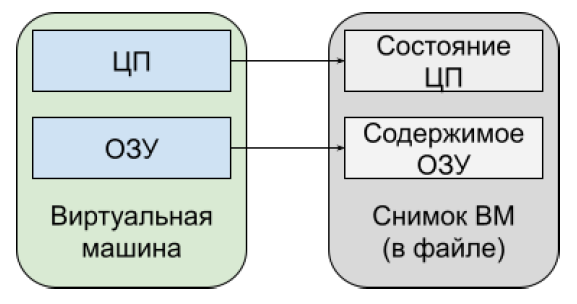
\includegraphics[width=1\textwidth]{4.png}}\\
    \label{framework} 
\end{figure}

Одна из интересных особенностей виртуальных машин заключается в том, что их полное состояние
можно легко зафиксировать и сохранить, чтобы потом это состояние можно было использовать как
минимум для нескольких интересных трюков:

\begin{itemize}
    \item создание так называемых снимков, то есть сохранение состояния ВМ в некоторый момент
    времени;
    \item копирование ВМ для их распространения или сохранения резервной копии;
    \item перенос ВМ с одного компьютера на другой, в том числе между компьютерами с разными
    хозяйскими ОС.
\end{itemize}

Действительно, если остановить исполнение виртуальной машины в некий момент времени, то её
полное состояние будет состоять из:

\begin{itemize}
    \item состояния виртуального процессора или процессоров;
    \item состояния прочей используемой аппаратуры (виртуального монитора, сетевого и
    USB-контроллера и т.д.);
    \item содержимого оперативной памяти;
    \item содержимого дискового накопителя.
\end{itemize}

Первые три пункта доступны в виде структур данных гипервизора, а содержимое накопителя
находится или в файле на файловой системе хозяйской системы (вариант по умолчанию), или на
разделе реального диска. Так что сохранение всего состояния ВМ не составляет большой проблемы.
Однако могут возникнуть следующие сложности:

\begin{enumerate}
    \item \textbf{Большой объём данных, которые нужно сохранить.} Представь те себе несколько гигабайт
    оперативной памяти и ещё несколько десятков гигабайт дискового накопителя. Немного
    упрощает ситуацию тот фтак , что количество места, которое виртуальный накопитель
    занимает на реальном диске системы, фактически соответствует том у , насколько он заполнен
    данными. Всег да следует помнить, что при работе с данными их объём сильно коррелирует с
    временем, требующимся для их обработки. Причём не всег да зависимость линейная. Чем
    «дальше» находится память от процессора и чем она медленнее, тем больше времени
    процессор находится в ожидании загрузки или выгрузки данных, не говоря о времени,
    затраченном на собственно обработук . В свою очередь, чем больше объём данных, тем в
    более медленной и «далёкой» памяти эти данные обычно находятся.
    \item \textbf{Необходимость в дополнительных действиях со стороны пользователя при
    нестандартных конфигурациях виртуальной машины.} Например, если для хранения
    данных ВМ используется реальный раздел на диске хозяйской системы, то необходимо
    создать его бинарную копию. Данная ситуация усугубляется ещё и тем, что нельзя сделать
    бинарную копию только части раздела, даже если он используется частично. Разумеется,
    можно созданную бинарную копию упаковать архиватором и благодаря этому избавиться от
    бесполезного объёма, заполненного нулями. Но всё равно сначала нужно сделать слепок
    всего раздела, который может занимать десятки или сотни гигабайт, разместить его на
    каком-то локальном хранилище (мы же не хотим по сети передавать такие объёмы данных) и
    лишь затем сжать его в архив. То есть требуется ещё больше места на диске хозяйской
    системы, а также достаточно много времени на создание бинарной копии и её архивирование.
\end{enumerate}

Тем не менее не всегда требуется создавать полную копию всего состояния ВМ. Если полная копия
однажды сделана, то для фиксации состояния ВМ в следующий момент времени достаточно
сохранить разницу с предыдущим сохранённым состоянием. Именно эта особенность используется
при итеративном создании снимков (англ. snapshot). Благодаря этому можно с лёгкостью сохранять
множество состояний ВМ для последующего возврата к одному из предыдущих состояний. Поскольку
требуется сохранить очень небольшое количество данных, это будет происходить быстро и потребует
незначительного объёма локального накопителя.\\

При использовании инкрементальных снимков есть одна неочевидная проблема: нельзя просто так
избавиться от какого-то одного снимка, потому что он используется для создания следующего. При
восстановлении из какого-то снимка все предыдущие снимки будут последовательно наложены
поверх самого последнего полного состояния. А потому правильное удаление одного промежуточного
снимка должно производиться при помощи специальной утилиты (как правило, доступной в комплекте
с гипервизором), которая внесёт необходимые изменения в оставшиеся снимки. Например,
интегрирует изменения, сохранённые в удаляемом снимке, с последующим. И тут может выясниться,
что дополнительное место на локальном накопителе освободить не удалось, а времени и
электричества на перегенерацию оставшихся снимков ушло очень много.\\

С последним снимком таких проблем нте , потому что от него не зависит следующий, так что
последний снимок может быть запросто удалён.

\subsubsection*{Переносимость между хозяйскими системами}
\addcontentsline{toc}{subsubsection}{Переносимость между хозяйскими системами}

Ещё одна возможность, открывающаяся благодаря сохранению полного состояния ВМ, — перенос ВМ
между хозяйскими системами, то есть между разными компьютерами. В данном случае речь идёт о
ситуации, когда на обоих компьютерах установлен один и тот же гипервизор. Таким образом возможно
передать результаты своей работы кому-то или же использовать чьи-то наработки. Или же, сохраняя
состояние ВМ на переносном накопителе, таком как SD-карты или USB-привод, можно буквально
перемещаться со своей виртуальной машиной с одного компьютера на другой и всегда работать в
известном, удобном и безопасном окружении.

\subsubsection*{Совместимость между виртуальными машинами разных
производителей}
\addcontentsline{toc}{subsubsection}{Совместимость между виртуальными машинами разных
производителей}

Теоретически ничто не должно мешать переносу ВМ между разными гипервизорами (по крайней мере,
одного типа), так как копия содержимого памяти и накопителя по большому счёту мало зависит от
гипервизора. Это же просто линейный буфер с данными. Состояния процессора вроде бы тоже
должны быть одинаковыми, если используются одинаковые модели процессоров. Мы же помним, что
состояние процессора описывается всего лишь содержанием его регистров. Фактически единственная
переносимая между гипервизорами субстанция — это содержимое виртуального дискового
накопителя. Неприятное следствие такого ограничения состоит в том, что переносить можно только
остановленные или «выключенные» виртуальные машины, всё состояние которых состоит из образа
дискового накопителя, так как состояния процессора и оперативной памяти не имеют значения.\\

Более того, к сожалению, каждый разработчик гипервизора предпочитает использовать своё
представление виртуального диска. Причём не всегда желая поддерживать альтернативные
варианты. VMware использует для работы исключительно формат VMDK (сокр. от англ. Virtual Machine
DisK). То есть образы дисков, созданные другими гипервизорами, необходимо конвертировать в
формат VMDK перед использованием с гипервизорами VMware, что не добавляет пользователю
удобства. В этом смысле Oracle Virtualbox более удобен, так как может использовать образы дисков в
«чужих» форматах. Тем не менее, только использование «своего» для гипервизора формата
представления виртуального диска даёт возможность получить все преимущества данного
гипервизора.

\subsubsection*{Производительность}
\addcontentsline{toc}{subsubsection}{Производительность}

Ввиду того, что гипервизор второго типа работает поверх ОС хозяйской системы, можно сделать
предположение, что эффективность такого гипервизора будет не очень высокой из-за значительных
накладных расходов на использование сервисов хозяйской ОС. Особенно интересно сравнить
производительность гипервизоров разного типа от одного производителя. В частности, VMware
Workstation Pro/Player и VMware ESXi, поскольку оба гипервизора используют некоторое количество
одинаковых компонентов и оптимизаций.\\

Ниже приведены измерения, выполненные при помощи Phoronix Test Suite на компьютере Intel
NUC8I5BEK c процессором Intel Core i5-8259U (4 ядра, 8 потоков), оснащённом 16 Гбайт ОЗУ и SSD
Samsung 970 Evo. Во всех случаях использовался Linux-дистрибутив Ubuntu 18.04.3 с ядром
5.0.0-25-generic (соответствует версии 5.0.18 с \href{www.kernel.org}{www.kernel.org}) и компилятором GCC 7.4.0.\\

\textbf{Использовались следующие системы:}

\begin{enumerate}
    \item Без гипервизора:
    \begin{enumerate}
        \item[a.] хозяйская система Intel NUC8I5BEK. 
    \end{enumerate}
        
    \item С гипервизором без хозяйской ОС:
    \begin{enumerate}
        \item[a.] гипервизор первого типа VMware ESXi 6.7. 
    \end{enumerate}

    \item С гипервизором поверх хозяйской системы с ОС Ubuntu:
    \begin{enumerate}
        \item[a.] гипервизор второго типа VMware Workstation Player;
        \item[b.] гипервизор второго типа Oracle VirtualBox.
    \end{enumerate}
         
\end{enumerate}

\textbf{Для оценки производительности использовались следующие тесты:}
\begin{enumerate}
    \item Измерение производительности оперативной памяти при помощи \\RAMspeed/SMP.
    \item Декодирование видеопотока из формата H.264.
    \item Сжатие данных архиватором 7zip.
    \item Измерение длительности полной компиляции ядра ОС Linux.
    \item Обслуживание запросов веб-сервером Apache.
\end{enumerate}

\newpage

\begin{figure}[h]
    \centering
    \scalebox{1}{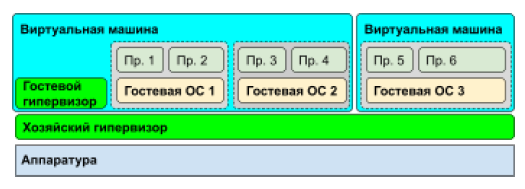
\includegraphics[width=1\textwidth]{5.png}}\\
    \label{framework} 
\end{figure}

\begin{figure}[h]
    \centering
    \scalebox{1}{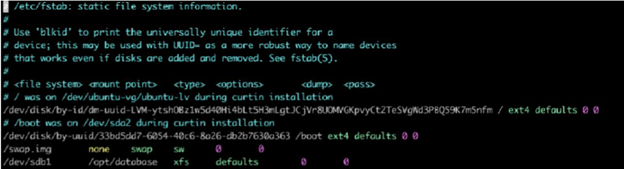
\includegraphics[width=1\textwidth]{6.png}}\\
    \label{framework} 
\end{figure}

\newpage

\begin{figure}[h]
    \centering
    \scalebox{1}{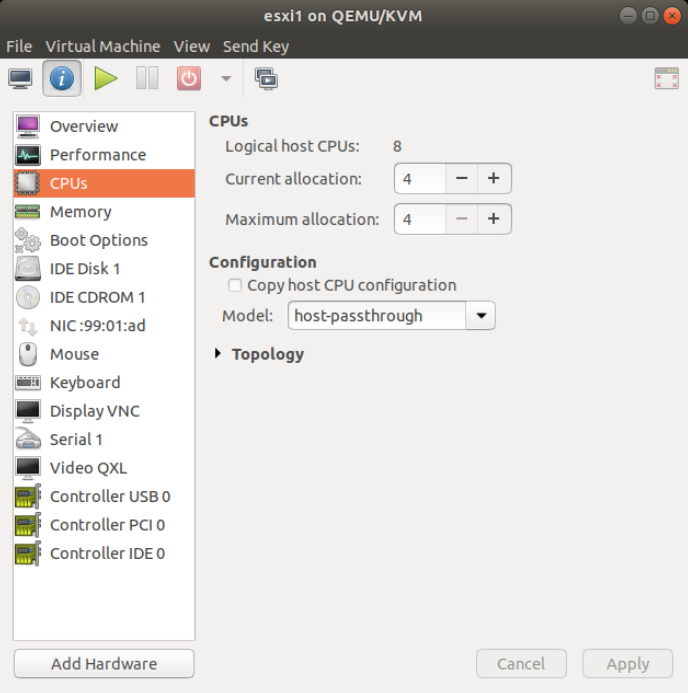
\includegraphics[width=1\textwidth]{7.png}}\\
    \label{framework} 
\end{figure}


Как можно видеть из резуль татов измерений, некоторое количество нагрузок обрабатывается любым
гипервизором не хуже, чем непосредственно хозяйской системой.\\

В частности, работа с памятью (тест RAMspeed) происходит практически с одинаковой скоростью. Это
и не удивительно: все участвовавшие в сравнении гипервизоры выполняют код гостевых систем
непосредственно на хозяйском процессоре, без какой-либо бинарной трансляции. Работа с памятью,
по крайней мере, последовательное или линейное чтение и запись, не вызывает частых событий,
например, отказов страниц, требующих переключения в контекст гипервизора.\\

Сжатие данных, перекодирование видеофайла и компиляция ядра Linux показывают некоторое
отставание в скорости работы гипервизоров по сравнению с исходной системой. Причём при данных
нагрузках уже становятся видны некоторые преимущества гипервизора первого типа (VMware ESXi и
KVM) перед обоими гипервизорами второго типа (VMware Workstation Player и Oracle VirtualBox).\\

Тем не менее разница между гипервизорами разного типа, а также хозяйской системой едва заметна,
потому что основное время тратится на обработку данных в памяти. А наблюдаемое отставание от
хозяйской системы обусловлено тем, что в отличие от операций с оперативной памятью, в данных
тестах (компрессия данных при помощи 7zip, декодирование видеопакетом кодеков FFMPEG и
компиляция ядра Linux) происходит весьма интенсивная работа с дисковым накопителем, что, в свою
очередь, требует вовлечения гипервизора.\\

А вот тест с веб-сервером Apache демонстрирует совершенно другую картину. Результаты
гипервизора первого типа (VMware ESXi) оказываются близки к результатам хозяйской системы, в то
время как оба гипервизора второго типа существенно отстают, показывая вдвое меньшие результаты.
Скорее всего, это обусловлено тем, что для обслуживания каждого запроса веб-сервер создаёт новый 
процесс, что требует существенной вовлечённости гипервизора для обработки большого количества
отказов страниц.\\

Новый процесс запускается в своём собственном адресном пространстве, а потому ранее
установленные настройки устройства управления виртуальной памятью (MMU) оказываются
неприменимы и их нужно устанавливать заново для каждой новой страницы памяти.

\subsubsection*{Типовые сферы применения}
\addcontentsline{toc}{subsubsection}{Типовые сферы применения}

Как уже упоминалось ранее, гипервизоры второго типа в основном используются для виртуализации
рабочих мест (десктопа). То есть они создают модель персонального компьютера, на которой может
быть запущена полноценная ОС, как отличающаяся от хозяйской, так и совпадающая с ней.\\

Причин для создания виртуального рабочего места может быть довольно много, например:

\begin{enumerate}
    \item \textbf{Создание контролируемого окружения для тестирования и оценки производительности
    ПО.} Для этого особенно удобно использовать сохранённое состояние ВМ (снимок). Можно при
    каждом новом запуске, с одной стороны, иметь все необходимые настройки уже
    применёнными, в отличие от новой установки и конфигурации системы перед каждым
    запуском. С другой стороны, можно всег да иметь совершенно одинаковые начальные условия,
    таким образом получая сравнение «яблок с яблоками». Английское выражение compare apples
    to apples означает сравнение сопоставимых субстанций.
    \item \textbf{Создание сильно ограниченной песочницы для исследования поведения ПО и системы
    в целом.} В виртуальной машине можно безопасно запускать ПО, заражённое вирусами, и
    исследовать их поведение, не рискуя потерять важную информацию, имеющуюся в хозяйской
    системе.
    \item \textbf{Запуск ОС, отличной от хозяйской.} Самые распространённые случаи — это запуск гостевой
    системы с Linux-дистрибутивом на компьютере с Windows и наоборто . Хотя возможны
    варианты запуска разных версий одной и той же ОС: гостевой системы с Windows 7 на
    компьютере с Windows 10, гостевой системы с дистрибутивом Debian или CentOS на
    компьютере с Ubuntu.
    \item \textbf{Подготовка и распространение готового окружения для запуска какого-то ПО.} Таким
    образом можно обеспечить воспроизведение проблем, обнаруженных пользователями. ВМ, в
    которой пользователь воспроизвёл проблем у , передаётся разработчикам для дальнейших
    исследований. Или однажды настроенная опытным инженером среда разработки может быть
    использована начинающими без необходимости перед началом работы выполнять сложную
    настройку системы и ПО.
\end{enumerate}

\section*{Примеры реализации}
\addcontentsline{toc}{section}{Примеры реализации}

После обзора особенностей, характерных для всех гипервизоров второго типа, мы готовы
рассмотреть конкретные реализации на примере двух самых распространённых гипервизоров такого
типа: VMware Workstation Pro/Workstation Player/Fusion for Mac и Oracle Virtualbox. Также мы
рассмотрим эмулятор широкого спектра аппаратуры QEMU в режиме гипервизора второго типа, то
есть без поддержки KVM. Этот обзор подготовит вас к использованию такого рода гипервизоров
практически в любой ситуации.

\subsection*{VMware Workstation Pro, VMware Workstation Player и
VMware Fusion}
\addcontentsline{toc}{subsection}{VMware Workstation Pro, VMware Workstation Player и
VMware Fusion}

Начнём мы разговор с продуктов компании VMware. Она, дав толчок развитию и становлению рынка
виртуализации рабочих мест, стала неоспоримым лидером на рынке коммерческих систем
виртуализации. Причём виртуализации не только рабочих мест, но и серверов.\\

Гипервизоры второго типа компании VMware представлены на рынке в виде трёх продуктов,
незначительно отличающихся друг от друга. Все они предназначены для запуска на современных
64-битных процессорах Intel.\\

\begin{enumerate}
    \item \textbf{Workstation Pro} — флагманский гипервизор второго типа от VMware. Может быть запущен в
    системе с 64-битными ОС Windows (начиная с Windows 7) и современными
    Linux-дистрибутивами, такими как Ubuntu (начиная с версии 15.04), Red Hat Enterprise Linux 6 и
    более новыми, и некоторыми другими дистрибутивами. Workstation Pro поддерживает
    создание снимков ВМ и их клонирование, одновременный запуск нескольких ВМ, а также
    может быть интегрирован в VMware vSphere — платформу для виртуализации
    ИТ-инфраструктуры предприятия.
    \item \textbf{Workstation Player} — это версия гипервизора Workstation Pro. Она имеет некоторые
    ограничения, зато доступна для бесплатного использования в личных целях. Особенности,
    перечисленные выше для Work- station Pro, недоступны в Workstation Player: нет возможности
    создавать снимки и клоны ВМ, запускать несколько ВМ одновременно и интегрировать ВМ в
    VMware vSphere.
    \item \textbf{Fusion for Mac} — аналог Workstation для компьютеров Apple Macin- tosh с процессорами Intel.
    Существует в двух версиях Fusion и Fusion Pro, которые несколько отличаются
    поддерживаемыми возможностями. При этом важно отметить, что на настоящий момент
    (VMware Fusion 11) не существует бесплатной версии Fusion, аналогичной Work- station Player
    для Windows. Есть только возможность воспользоваться бесплатным тестовым периодом.
\end{enumerate}

Поскольку обозначенные выше продукты VMware имеют закрытые исходные коды, невозможно
провести точный и подробный анализ внутреннего устройства всех этих продуктов. Приходится
полагаться на доступные крупинки информации, опубликованные компанией-разработчиком, уповать
на здравый смысл и академические исследования. Мы можем сделать предположение, что все
названные гипервизоры используют одно и то же ядро гипервизора, а их отличия сводятся к
специфической интеграции с хозяйской системой (Windows, Linux или macOS), а также ограничению
дополнительных возможностей в бесплатных или более дешёвых версиях (VMware Workstation Player
и VMware Fusion).

\subsubsection*{Тип виртуализации}
\addcontentsline{toc}{subsubsection}{Тип виртуализации}

Мы уже многократно упоминали, что все упомянутые выше продукты — это гипервизоры второго типа,
то есть они работают поверх хозяйской ОС и активно пользуются её сервисами. Запуск 32-битных
гостевых ОС возможен на процессорах, не имеющих поддержки аппаратной виртуализации (Intel VT-x,
AMD-V). Соответственно, в отсутствие поддержки аппаратной виртуализации гипервизор VMware
осуществляет адаптивную бинарную трансляцию кода гостевой системы, позволяя выполнять
безопасные части кода гостевой системы непосредственно на реальном процессоре системы. Такой
подход, как ни странно, обеспечивает весьма высокую эффективность гипервизора. Это связано с
тем, что команды, требующие интерпретации, встречаются относительно редко. Их интерпретация
зачастую выполняется гораздо быстрее, чем переключение между режимами гостя и гипервизора в
случае использования аппаратной поддержки виртуализации. Однако 64-битные гостевые системы
требуют наличия включённой аппаратной виртуализации в хозяйской системе.\\

Что касается виртуализации устройств ввода-вывода, то гипервизор VMware по умолчанию
предлагает эмуляцию некоторых стандартных уст- ройств, таких как сетевой контроллер (в зависимости
от типа гостевой ОС, AMD PCnet или Intel E1000), PS/2-клавиатуры и USB-мыши. Также доступны
паравиртуализованные устройства, такие как усовершенствованные сетевые контроллеры vmxnet2 и
vmxnet3, имеющие большую производительность по сравнению с эмулируемыми вариантами. Однако
использование этих устройств гостевой системой становится возможно только после установки
набора расширений, кроме всего прочего содержащего драйвера тех самых дополнительных
устройств VMware Tools.\\

Графический интерфейс конфигурации VMware не даёт возможности выбрать тип сетевого
контроллера и устанавливает вариант, предусмотренный по умолчанию для выбранного типа гостевой
ОС. Потому для переключения типа сетевого контроллера необходимо вручную изменить файл
конфигурации ВМ (.vmx): параметр \colorbox{backcolour}{ethernetX.virtualDev} установить равным \colorbox{backcolour}{vmxnet3.} X в
названии параметра — это номер сетевого контроллера, начинающийся с 0, то есть при единственном
сетевом контроллере ВМ полное название параметра будет \colorbox{backcolour}{ethernet0.virtualDev}.

\subsubsection*{Состояние виртуальной машины}
\addcontentsline{toc}{subsubsection}{Состояние виртуальной машины}

Полное состояние ВМ описывается файлами в рабочей директории. Для хозяйской системы Windows
это обычно будет папка с названием виртуальной машины в \colorbox{backcolour}{\%homepath\%{\textbackslash}Documents{\textbackslash}Virtual Machines\textbackslash}, для хозяйской системы Linux — XXX, для MacOS — YYY, где содержатся:

\begin{itemize}
    \item .vmx — конфигурация ВМ;
    \item .vmx — конфигурация ВМ;
    \item .vmem — образ оперативной памяти, включая изменения с момента создания последнего
    снимка ВМ (существует только ког да ВМ запущена);
    \item .vmsn — состояние ВМ в момент создания снимка;
    \item .vmss — состояние ВМ при её приостановке;
    \item логи и дополнительные служебные данные.
\end{itemize}

Таком образом, при сохранении всего содержимого рабочей директории ВМ, её можно переносить не
только в пределах одного компьютера, но и между разными компьютерами. В том числе рабочую
директорию ВМ можно хранить на внешнем носителе, таком как SD-карта, USB-флеш-диск или
внешний диск, подключаемый любым способом: USB, Thunderbolt, eSATA и т. Д.

\subsubsection*{VMware Tools}
\addcontentsline{toc}{subsubsection}{VMware Tools}

Все продукты для виртуализации рабочих мест поддерживают интеграцию с хозяйской системой при
помощи VMwarTe ools. Благодаря VMwarTe ools появляются следующие возможности:

\begin{enumerate}
    \item Общий буфер обмена между хозяйской и гостевыми системами. Это позволяет легко
    переносить небольшие объёмы данных между ними. Например, фрагменты текстов, адреса
    веб-страниц и т.п.
    \item Становится возможно перемещать файлы между гостевой и хозяйскими системами, просто
    перетягивая их мышкой из окна гостя и обратно.
    \item Ещё один способ обмена файлами становится доступен при помощи HGFS (Host Guest File
    System) — специальной файловой системы, которая позволяет гостю получить доступ к
    указанным папкам хозяйской системы.
    \item Незаметное переключение указателя мыши между хозяйской и гостевой системами. То есть
    при попытке вывести указатель мыши за границы окна гостевой системы он автоматически
    возвращается в хозяйскую систему. В противном случае, то есть без установленных в гостевой 
    системе VMware Tools, для возврата указателя мыши из гостевой системы нужно использовать
    специальную комбинацию клавиш (по умолчанию Ctrl + Alt).
    \item Для ещё большей интеграции с хозяйским окружением предусмотрен режим Unity, который
    позволяет запускать приложения гостевой системы в отдельных окнах. Таким образом у
    пользователя создаётся ощущение, что приложения гостевой системы запускаются
    непосредственно в хозяйской системе.
\end{enumerate}

\subsubsection*{Дополнительные возможности}
\addcontentsline{toc}{subsubsection}{Дополнительные возможности}

Набор дополнительных возможностей гипервизоров VMware, доступный пользователю, сильно
отличается от продукта к продукту. Самый доступный вариант — VMware Workstation Player, которым в
личных целях можно пользоваться даже бесплатно, позволяет запускать только одну ВМ в один
момент времени, не поддерживает создание снимков и клонов ВМ. Что, однако, не отменяет
возможности создания нескольких ВМ и переключения между ними, останавливая или ставя на паузу
все, кроме одной.\\

Тем не менее VMware Workstation Player вполне годится для ознакомления с гипервизорами и
виртуальными машинами и использования ВМ для создания ещё одной полноценной системы.
Например, с ОС, отличающейся от хозяйской. Более того, производительность VMware Workstation
Player ни в чём не уступает более дорогим продуктам VMware для виртуализации десктопа.\\

Более функциональные продукты, такие как VMware Workstation Pro и VMware Fusion (Pro),
предоставляют дополнительные возможности, в частности:

\begin{enumerate}
    \item \textbf{Создание снимков ВМ для возможности «отката» к предыдущему состоянию.}
    \item \textbf{Клонирование ВМ для создания работоспособных копий ВМ.} Дело в том, что полную
    бинарную копию ВМ не удастся запустить одновременно с оригинальной ВМ. Причина в том,
    что их некоторые критически важные идентификаторы, такие как UUID ВМ и MAC-адреса
    виртуальных сетевых контроллеров, будут совпадать Это помешает не только нормальной
    работе гипервизора, но другим устройствам в сети.\\

    Причём, помимо полных, совершенно независимых друг от друга, клонов, можно создавать так
называемые связанные клоны (от англ. linked clone). По сути, связанный клон — это снимок
оригинальной ВМ, который можно исполнять одновременно с оригинальной ВМ. Преимущество
состоит в том, что вместо копирования всего состояния оригинальной ВМ (включая образ
оперативной памяти и виртуальные диски), используется полный снимок оригинала и только
изменения, созданные новым клоном, записываются в отдельные файлы. Таким образом, создание
связанных клонов происходит практически мгновенно и место на файловом накопителе хозяйской
системы используется гораздо более эффективно за счёт отсутствия дубликатов данных.

\item \textbf{Интеграция в платформу для виртуализации ИТ - инфраструктуры VMware vSphere.}
Благодаря этому становится возможным управление виртуальными машинами удалённо, из
одной централизованной консоли. Это значительно упрощает жизнь системным
администраторам на предприятиях.
\end{enumerate}

Стоит упомянуть, что VMware предоставляет VIX API, при помощи которого можно создавать свои
инструменты управления виртуальными машинами VMware Workstation Pro/Player и VMware Fusion. В
качестве примера такого инструмента предоставляется утилита vmrun.

\subsubsection*{Лицензии на гипервизоры VMware}
\addcontentsline{toc}{subsubsection}{Лицензии на гипервизоры VMware}

В случае использования виртуальных машин необходимо помнить, что программное обеспечение,
установленное в каждом экземпляре ВМ, может требовать отдельной лицензии, не говоря о том, что
некоторые программные продукты не могут быть использованы в ВМ по условиям лицензии. Это
одинаково относится к любым гипервизорам.\\

Гипервизоры второго типа компании VMware с точки зрения лицензирования можно разделить на две
группы.

\paragraph*{Коммерческие лицензии} \mbox{}\\
\addcontentsline{toc}{paragraph}{Коммерческие лицензии}

К первой группе с платной (или коммерческой) лицензией можно отнести все рассмотренные ранее на
этом занятии продукты VMware. Для полноценного использования после окончания пробного периода
(как правило, 30 дней) необходимо приобрести лицензию. Причём лицензия никак не привязывается к
конкретному компьютеру или ОС. При необходимости можно удалить ранее установленный продукт и
использовать лицензию заново при новой установке. Более того, лицензию на VMware Player и
Workstation Pro можно использовать для активации соответствующего продукта в обеих
поддерживаемых ОС: Windows и Linux.\\

Однако существует одно важное ограничение: лицензии привязаны к мажорной версии продукта. То
есть лицензия, приобретённая для VMware Workstation Player v12, не активирует VMware Workstation
Player v13. При необходимости лицензировать более новую версию продукта придётся либо купить
новую лицензию на новую версию, либо сделать обновление лицензии от более старой версии до
более новой. Также можно сделать downgrade лицензии на более свежую версию продукта до более
ранней. Но такая лицензия не будет подходить для более свежей версии продукта — нужно будет
выполнить процесс обновления лицензии. Ещё есть возможность обновить лицензию от Workstation
Player до Workstation Pro.

\paragraph*{Бесплатные лицензии} \mbox{}\\
\addcontentsline{toc}{paragraph}{Бесплатные лицензии}

К нашему счастью, компания VMware даёт возможность бессрочно бесплатно использовать VMware
Workstation Player для личных нужд и в образовательных целях. Чего вполне достаточно, чтобы
познакомиться с особенностями работы и использования виртуальной машины на персональном
компьютере. Что интересно, использование продуктов VMware некоммерческими организациями
требует приобретения полноценной лицензии.

\subsection*{Oracle VirtualBox} 
\addcontentsline{toc}{subsection}{Oracle VirtualBox}

\begin{figure}[h]
    \centering
    \scalebox{0.7}{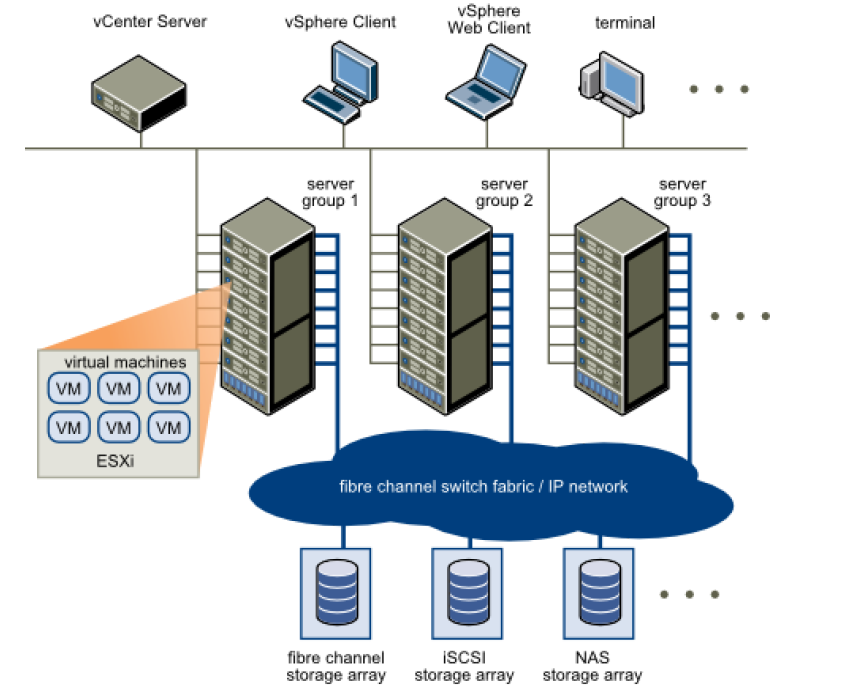
\includegraphics[width=1\textwidth]{8.png}}\\
    \label{framework} 
\end{figure}

\noindent Как мы помним из экскурса в историю, продукт под названием VirtualBox был изначально разработан
компанией InnoTek GmbH в середине двухтысячных, а 15 января 2007 года публике был представлен
InnoTek VirtualBox Open Source Edition (OSE) версии 1.3.2. Однако разработка началась задолго до
того, так как в руководстве пользователя ранних версий (например, Sun VirtualBox User Manual version
3.1.8) можно видеть упоминание версии 1.0.37, выпущенной 12 апреля 2005 года. Возможно, версии
до 1.3.2 никог да не были доступны вне компании InnoTek.\\

Очень возможно, что инженеры Innotek были вдохновлены работой над Connectix Virtual PC, когда они
адаптировали Virtual PC для операционной системы OS/2. Кроме того, первый широко
распространённый гипервизор второго типа VMware Workstation уже к 2005 году достиг в своём
развитии версии 5.0. Так что определённо инженерам Innotek было на что посмотреть и о чём
подумать, создавая весьма интересную и сильную альтернативу продукту, захватившему к тому
времени существующий рынок виртуализации персонального компьютера. А потому не приходится
удивляться, что в смысле используемых технических решений VirtualBox очень близок к VMware
Workstation и Fusion.\\

Существенные различия между продуктами Oracle и VMware стоит искать в плоскости
дополнительных возможностей бесплатных версий продуктов и интеграции в корпоративную
инфраструктуру (VMware vSphere, Oracle VBoxHeadless).\\

Ещё одно важное отличие продуктов Oracle от продуктов компании VMware состоит в том, что все
компоненты VirtualBox, кроме Extension Pack, доступны в исходных кодах, а это значит, что любой
желающий может удовлетворить своё любопытство насчёт реализации тех или иных особенностей.
Более того, существует публичный трекер проблем, где можно сообщать об обнаруженных
проблемах, но ещё важнее возможность найти описание или даже решение своей нынешней
проблемы. Кроме того, есть весьма подробная техническая документация, которая освещает вопросы
устройства самого гипервизора, описывает шаги для самостоятельной сборки, а также тонкой
настройки различных компонентов гипервизора и инструментов для работы с ним.\\

Однако открытые исходные коды имеют и ещё одно существенное достоинство. Благодаря их
открытости специалисты по информационной безопасности, равно как и все желающие, могут
проводить независимый аудит и изучение исходных кодов на предмет наличия уязвимостей.\\

Как и конкурирующий гипервизор от компании VMware, VirtualBox используется для виртуализации
компьютеров на базе процессоров с архитектурой x86. Причём первоначально поддерживались
только 32-битные процессоры или 64-битные процессоры в 32-битном режиме. Но, начиная с версии
5.0, поддержка хозяйских 32-битных процессоров была прекращена. На сегодняшний день запуск
VirtualBox возможен только на 64-битных процессорах семейства x86 производства AMD и Intel. При
этом, разумеется, всё ещё остаётся возможность запуска гостевых 32-битных ОС.\\

Используются такие же режимы работы гипервизора: программная виртуализация, то есть работа без
использования аппаратного ускорения виртуализации, и аппаратная виртуализация с использованием
Intel VT-x или AMD-V, причём для запуска 64-битных гостевых систем используется только последний
режим.\\

В случае использования программной виртуализации пользовательское ПО гостевой системы
выполняется непосредственно процессором точно так же, как и в отсутствие гипервизора: raw-mode,
режим без изменений в терминологии VirtualBox. Ядро гостевой ОС выполняется в первом круге
безопасности вместо нулевого, в котором работают ядро хозяйской ОС и гипервизор. Но для
повышения эффективности работы гипервизора код гостевой системы анализируется на лету.
Инструкции, которые могли бы вызвать передачу управления гипервизору для работы с устройствами
ввода-вывода, управления прерываниями или подсистемой виртуальной памяти, при возможности
подменяются кодом, реализующим необходимую функциональность, не покидая первого круга
защиты. Для этого используются дизассемблер и рекомпилятор, которые были позаимствованы из
другой системы виртуализации с открытым кодом — QEMU.\\

Режим аппаратной виртуализации использует новые режимы работы процессоров Intel и AMD.
Во-первых, для более полного и надёжного разделения хозяйской и гостевых систем, а во-вторых, для 
предоставления возможности гостевым системам выполнять некоторые привилегированные команды
самостоятельно, без дополнительных вызовов гипервизора.\\

В настоящее время ведётся работа над добавлением поддержки паравиртуализованных
интерфейсов, предоставляемых ОС, в которой запущен гипервизор. В частности, при запуске
гипервизора в системах с ОС Linux, VirtualBox может использовать предоставляемые KVM
паравиртуализованные часы и spinlock. При запуске под ОС Windows поддерживаются некоторые
возможности, предоставляемые Microsoft Hyper-V, такие как часы, отладка гостевых систем и
некоторые другие. Возможно, со временем мы будем наблюдать большую интеграцию с
гипервизорами, предоставляемыми хозяйскими ОС.\\

Что касается устройств ввода-вывода, Oracle VirtualBox эмулирует их большую часть, за исключением
сетевого контроллера Virtio-net, с одной стороны, предоставляющего стандартный Virtio-интерфейс
гостевой системе, а с другой стороны, эффективно использующего сетевой интерфейс хозяйской
системы. Тем самым он значительно снижает затраты на, в общем-то, бессмысленную эмуляцию
реального сетевого контроллера, такого как AMD PCNet или Intel PRO/1000. Однако, во-первых, для
использования Virtio устройств необходимо установить соответствующие драйверы на хозяйской
системе. А во-вторых, думается, мало кому придёт в голову для высокоскоростной работы с сетью
использовать систему виртуализации десктопа.

\subsection*{Особенности гипервизора Oracle VirtualBox} 
\addcontentsline{toc}{subsection}{Особенности гипервизора Oracle VirtualBox}

\subsubsection*{Поддержка хозяйских и гостевых систем} 
\addcontentsline{toc}{subsubsection}{Поддержка хозяйских и гостевых систем}

Будучи ПО с открытыми исходными кодами, VirtualBox со временем оказался портирован на
большинство ОС общего назначения, в частности, Linux, Windows, Solaris, macOS и FreeBSD. Причём
на всех перечисленных ОС используется один и тот же продукт, в то время как VMWare Workstation
существует только для Linux и Windows. А в macOS необходимо устанавливать формально
совершенно другой продукт — VMware Fusion, хотя фактически он ничем не отличается от
Workstation.\\

Список гостевых систем совпадает с тем, что поддерживают продукты VMware: Linux, Windows,
Solaris, FreeBSD, macOS. Снова с оговоркой, что формально macOS можно запустить только в
VMware Fusion или Oracle VirtualBox на компьютере Apple.\\

Вообще говоря, это не ограничение VMware Fusion, а требование лицензии на macOS запускать
macOS исключительно на аппаратуре Apple, неважно, на реальной аппаратуре или в виртуальной
машине. С технической же точки зрения macOS можно было бы запустить и в VMware Workstation на
системе с ОС Linux или Windows.\\

Хотя если на компьютер производства Apple установить Windows или виртуальную машину с
Windows, то формально станет возможным запуск macOS в VMware Workstation.

\subsubsection*{Состояние виртуальной машины} 
\addcontentsline{toc}{subsubsection}{Состояние виртуальной машины}

Файлы, описывающие состояние виртуальной машины Oracle VirtualBox, хранятся в папке, указанной
при создании виртуальной машины. По умолчанию в домашней директории пользователя создаётся
папка VirtualBox VMs, в которой создаются папки индивидуальных виртуальных машин. Например,
файлы виртуальной машины под названием Ubuntu будут храниться:

\begin{itemize}
    \item в хозяйской системе с Windows: \colorbox{backcolour}{C:\textbackslash Users\textbackslash username\textbackslash VirtualBox VMs\textbackslash} \\ \colorbox{backcolour}{Ubuntu};
    \item в случае Linux: \colorbox{backcolour}{/home/username/VirtualBox VMs/Ubuntu};
    \item на macOS: \colorbox{backcolour}{/Users/username/VirtualBox VMs/Ubuntu}.
\end{itemize}

Состояние виртуальной машины в простейшем случае (машина выключена) состоит из её
конфигурации, содержащейся в файле с расширением .vbox, и образа диска, хранящегося по
умолчанию в файле с расширением .vdi. При создании снимка виртуальной машины VirtualBox
создаёт новый образ диска, хранящий только разницу, возникшую с момента создания снимка, а
также полную бинарную копию оперативной памяти гостевой системы и состояния всех её
виртуальных процессоров и прочих виртуализованных устройств в файле с расширением .sav.\\

Интересно, что постановка виртуальной машины на паузу по сути равнозначна созданию снимка без
необходимости сохранять изменения образа диска, то есть создаётся только файл с расширением
.sav. А потому постановка на паузу виртуальной машины сразу же после создания снимка происходит
мгновенно и не требует никаких дополнительных действий от гипервизора: все состояния уже
сохранены на диске хозяйской системы.

\subsubsection*{VirtualBox Extension Pack} 
\addcontentsline{toc}{subsubsection}{VirtualBox Extension Pack}

Базовая версия Oracle VirtualBox, будучи бесплатной и не имея каких-либо ограничений на её
использование в личных, коммерческих и любых других целях, обладает некоторыми ограничениями
функциональности. Однако, установив VirtualBox Extension Pack, распространяемый под
проприетарной лицензией, накладывающей ограничения на коммерческое использование, можно
получить дополнительные удобства:

\begin{itemize}
    \item поддержку устройств USB 2.0 и 3.0;
    \item шифрование образов дисковых накопителей;
    \item доступ к виртуальной машине при помощи протокола VRDP (расширенная Oracle, но при этом
    обратно совместимая версия протокола Microsoft RDP);
    \item возможность установки по сети при помощи Intel PXE.
\end{itemize}

Пожалуй, для индивидуального использования интерес представляет только поддержка
высокоскоростных USB-устройств, остальное более важно для корпоративного использования.

\subsubsection*{VirtualBox Guest Additions} 
\addcontentsline{toc}{subsubsection}{VirtualBox Guest Additions}

Существует комплект улучшений для гостевых систем Oracle VirtualBox, при использовании которых
ощутимо повышается интеграция хозяйской и гостевых систем, что делает работу с виртуальной
машиной более комфортной и зачастую более продуктивной.

\subsubsection*{Управление виртуальными машинами} 
\addcontentsline{toc}{subsubsection}{Управление виртуальными машинами}

Существенное отличие от продуктов VMware, особенно Workstation Player, состоит в возможности
гибкого управления виртуальными машинами, причём даже в базовой версии. Напомним, что VMware
Workstation Player позволяет в один момент времени иметь запущенной только одну виртуальную
машину, не позволяет создавать клоны, а также делать снимки виртуальных машин. Oracle VirtualBox
не имеет таких ограничений и в этом смысле сопоставим по возможностям с VMware Workstation Pro.
Более того, виртуальными машинами VirtualBox возможно управлять при помощи разнообразных
фронтендов благодаря наличию открытого и хорошо документированного Main API.

\subsubsection*{Доступные варианты} 
\addcontentsline{toc}{subsubsection}{Доступные варианты}

\begin{enumerate}
    \item \textbf{Графический интерфейс пользователя} — самый очевидный способ управления
    виртуальной машиной, мало чем отличающийся от VMware Workstation или Fusion.
    \item \textbf{VBoxManage} — утилита управления из командной строки.
    \item \textbf{VBoxShell} — оболочка на языке Python.
    \item \textbf{VBoxSDL} — упрощённый графический интерфейс пользователя, реализованный при помощи
    SDL.
    \item \textbf{VBoxHeadless} — инструмент запуска виртуальных машин без вывода изображения на
    виртуальный монитор гостевой системы. При необходимости изображение с виртуального
    монитора может быть доступно при помощи любого RDP-клиента. Таким образом можно
    запускать виртуальные машины на удалённом сервере.
    \item \textbf{phpVirtualBox} — веб-интерфейс для управления виртуальными машинами Oracle VirtualBox.
\end{enumerate}

\textbf{SDL (Simple DirectMedia Layer)} — это свободная кроссплатформенная мультимедийная библиотека,
реализующая единый программный интерфейс к графической подсистеме, звуковым устройствам и
средствам ввода для широкого спектра платформ.\\

Дополнительно к имеющимся инструментам и утилитам можно создавать свои, используя удобные
библиотеки вроде pyvbox.\\

Стоит заметить, что всё это великолепие, за исключением VBoxHeadless, использующего VRDP,
который является частью VirtualBox Extension Pack, доступно даже в базовой бесплатной версии
VirtualBox, в отличие от продуктов VMware.

\subsubsection*{Лицензия} 
\addcontentsline{toc}{subsubsection}{Лицензия}

Начиная с версии 1.3.2, выпущенной в начале 2007 года, и до версии 3.0, выпущенной в конце 2010
года, существовали две разные версии VirtualBox:

\begin{enumerate}
    \item \textbf{Oracle VirtualBox} с проприетарной лицензией Personal Use and Eva- luation License (PUEL),
    дававшей право на использование в личных и образовательных целях. Чем-то напоминает
    лицензию на VMware Workstation Player.
    \item \textbf{VirtualBox Open Source Edition (OSE)}, которая имела ограниченный набор возможностей,
    зато распространялась под лицензией GPL.
\end{enumerate}

Начиная же с версии 4.0, выпущенной в декабре 2010 года, существует только одна версия VirtualBox,
которая во многом похожа по своим возможностям на ранее доступную версию OSE. Но её
возможности могут быть расширены за счёт дополнительно загружаемых модулей, в частности,
Oracle VM VirtualBox Extension Pack (распространяемого также под лицензией PUEL).\\

Что интересно, вплоть до девятой версии лицензия PUEL под «личным» использованием
подразумевала факт того, что пользователь сам скачал, установил и использует VirtualBox, включая
удалённое использование при помощи VNC или RDP. То есть отдельно не оговаривались условия
использования продукта в интересах бизнеса. Речь идёт о версии именно лицензии VirtualBox
Personal Use and Evaluation License (PUEL), а не о версии Oracle VirtualBox.\\

А вот десятая версия PUEL, обнародованная 20 июля 2017 года, добавила уточнение о
некоммерческом личном использовании. Так что в этом смысле Oracle VirtualBox снова оказался на
равных с конкурирующим продуктом от VMware.\\

Для коммерческого использования VirtualBox Extension Pack необходимо приобретение лицензии
Oracle VM VirtualBox Extension Pack Enterprise. Существенное отличие от продуктов VMware состоит в
том, что невозможно приобрести одну-единственную лицензию VirtualBox Extension Pack Enterprise.
На сегодняшний день минимальное количество таких лицензий, доступное для заказа, равно 100. Что
определённо не подходит для малого бизнеса или индивидуального использования в коммерческих
целях. Стоит это иметь в виду!

\section*{Практическое задание}
\addcontentsline{toc}{section}{Практическое задание}

\begin{enumerate}
    \item У становить VMware Workstation Player (или VMware Fusion, если в качестве хозяйской ОС
    используется macOS) и Oracle VirtualBox. В них запустить гостевую ОС на свой выбор.
    Убедиться, что работают базовые приложения: текстовый редактор и веб-браузер.
    \item * В любом из упомянутых гипервизоров запустить гостевую ОС с отключённой поддержкой
    виртуализации (AMD-V или Intel VT-x).
    \item * Произвести измерения производительности гипервизоров на своей системе при помощи
    PhoroniTx est Suite.
\end{enumerate}

\section*{Используемые источники}
\addcontentsline{toc}{section}{Используемые источники}

\begin{enumerate}
    \item \textit{A Comparison of Software and HardwareT echniques for x86 Virtualization}, Keith Adams, Ole
    Agesen, VMware.
    \item \textit{Oracle VM VirtualBox User Manual, Chapter 10T. echnical Background}, Oracle Corporation.
    \item \textit{VMware vs. Virtual Box: Comprehensive Comparison}, Michael Bose.
\end{enumerate}

\end{document}